\documentclass[useAMS,usenatbib,referee,12pt]{article}
\usepackage[margin=1.0in]{geometry}
\usepackage{amsmath}
\usepackage{amssymb}
\usepackage{amsfonts}
\usepackage{parskip}
\usepackage[round]{natbib}
\usepackage{color}
\usepackage[dvipsnames]{xcolor}
\usepackage{caption}
\usepackage{tabularx, booktabs}
\usepackage{float}
\usepackage{adjustbox}
\usepackage[toc,page]{appendix}
\usepackage{enumitem}
\usepackage{multirow}
\usepackage{setspace}
\doublespacing

\newcommand{\adam}[1]{{\color{blue} ADAM: #1}}
\newcommand{\jarad}[1]{{\color{Orange} #1}}
\newenvironment{indpar}[1]%
     {\begin{list}{}%
             {\setlength{\leftmargin}{#1}}%
             \item[]%
     }
     {\end{list}}

\newcommand{\vn}{\textbf{n}}
\newcommand{\vp}{\textbf{p}}
\newcommand{\vX}{\textbf{X}}
\newcommand{\vZ}{\textbf{Z}}
\newcommand{\vbeta}{\boldsymbol{\beta}}
\newcommand{\vxi}{\boldsymbol{\xi}}

\newcommand{\Exp}{\mbox{Exp}}
\newcommand{\Ga}{\mbox{Ga}}
\newcommand{\We}{\mbox{We}}
\newcommand{\LN}{\mbox{LN}}
\newcommand{\Po}{\mbox{Po}}
\newcommand{\Mult}{\mbox{Mult}}

\newcommand{\pdet}{p^{(det)}}
\newcommand{\ind}{\stackrel{ind}{\sim}}

\begin{document}

%\tableofcontents 

\begin{abstract}

Abundance estimates from animal point-count surveys require accurate estimates of detection probabilities.  
The standard model for estimating detection from removal-sampled point-count surveys assumes that organisms at a survey site are detected at a constant rate; however, this assumption is often not justified.  
%Detection rates can be influenced by organismal behaviors, survey methodology, and observer effort.  
%Failure to account for non-constant detection leads to biased estimates of detection and therefore of abundance.  
We consider a class of N-mixture model that allows for detection heterogeneity over time through a flexibly defined time-to-detection distribution (TTDD) and allows for fixed and random effects for both abundance and detection.
%We consider a class of N-mixture models that allow for detection heterogeniety through a mixture component, flexible two-parameter time-to-detection distributions (TTDDs), and allows for fixed and random effects for both abundance and detection.
%Whereas, under the standard approach, detection probability is modeled by dividing the observation period into equal-duration intervals, we instead model the detection {\it rate} in continuous time via a time-to-detection distribution (TTDD) embedded within a hierarchical N-mixture framework.  
Our model is thus a combination of survival time-to-event analysis with unknown-N, unknown-p abundance estimation.  
We specifically explore two-parameter families of TTDDs (e.g. gamma) that can additionally include a mixture component to model increased probability of detection in the initial observation period.
We find that modeling a TTDD by using a mixture component is necessary when data have a chance of arising from a distribution of this nature.
In addition, two-parameter distributions can outperform exponential-based models both when the truth is exponential or non-exponential.
Finally, we analyze an Overbird data set from the Chippewa National Forest using mixed effect models for both abundance and detection.
We demonstrate that the effects of explanatory variables on abundance and detection are consistent across mixture TTDDs but that flexible TTDDs result in lower estimated probabilities of detection and therefore higher estimates of abundance. 
%We find that modeling a TTDD by using a mixture component for increased probability of detection in the initial observation period is necessary when data have a chance of arising from distributions of this nature.
%In addition, the flexibility offered by two-parameter distributions, e.g. gamma, can outperform exponential based models when the truth is exponential or non-exponential.
%Finally, we analyze an Overbird data set from the Chippewa National Forest using mixed effect models for both abundance and detection and demonstrate that the effects of explanatory variables on abundance and detection are consistent across mixture TTDDs and that flexible TTDDs result in lower estimated probabilities of detection and therefore higher estimates of abundance. 
% We apply this model to Ovenbird counts from the Chippewa National Forest and to datasets simulated under different time-to-detection patterns.  
% Models assuming constant detection rates produce biased estimates of detection when true detection rates vary with time, whereas models allowing for variable detection (assuming gamma, Weibull, or lognormal distributed times to detection) produce less biased estimates of the detection probability and nominal credible interval coverage.  
% Models ignoring detection heterogeneity across subgroups yield biased estimates of detection when such heterogeneity exists, whereas models accounting for detection heterogeneity (modeled as a mixture) return reasonable coverage rates and can outperform heterogeneity-ignorant models even when there is no heterogeneity.

{\bf Keywords:} abundance; availability; N-mixture model; point counts; removal sampling; survival analysis; Bayesian

\end{abstract}

\newpage
\section{Introduction}\label{sec:intro}

Abundance estimates from animal point-count surveys require accurate estimates of detection probabilities.  
Removal sampling, where individuals are solely counted on their first capture, provides one established methodology for estimating detection probabilities \citep{Farnsworth2002}.
% cost-effective in that it requires neither multiple observers nor multiple site visits.
%Removal sampling is a species abundance surveying methodology in which observers capture and physically remove animals at a survey site over a series of trapping sessions.
%Assuming that individual capture rates remain constant over all trapping sessions, it is possible to estimate the proportion of individuals still not captured from the pattern of captures over time .  
%\citet{Farnsworth2002} adapted removal sampling to point-count surveys, suggesting that if: (i) observers record only the first time-to-detection for each animal, and (ii) times to first detection are interval-censored, then data will be similar in for to traditional removal sampled data.
%In the analysis of such data, the observation period is subdivided into unit intervals of equal duration, each of which is equivalent to a trapping session.
%Farnsworth's removal assumptions:\\
%(i) Closed population during survey\\
%(ii) no double-counting\\
%(iii) easy-to-detect group is entirely counted during first interval\\
%(iv) TTDD for hard-to-detect group is correct after the end of the observation period\\
%(v) if using limited radius counts, they are accurate
% Johnson2008: all birds present are available for detection
A typical assumption in removal sampling is a constant detection rate throughout the observation period, but this assumption is often unjustified \citep{Alldredge2007}. %\adam{Others, like Mantyniemi.}  
In particular, animal behaviors such as intermittent singing in birds and frogs or diving in whales \citep{Scott2005, Diefenbach2007, Reidy2011}, differences in behavior across subgroups of animals \citep{Farnsworth2005}, observer impacts on animal behaviors \citep{McSheaRappole1997, Rosenstock2002, Alldredge2007}, and variations in observer effort, e.g. lack of settling in period \citep{LeeMarsden2008, Johnson2008}, can all lead to time-varying rates of detection.
%In particular, animal behaviors, e.g. intermittent singing in birds and frogswhales \citep{Scott2005, Diefenbach2007, Reidy2011}, observer behaviors, e.g. pre-counting and disturbing species \citep{McSheaRappole1997, Rosenstock2002, Alldredge2007, LeeMarsden2008, Johnson2008}, and survey methodology, e.g. lack of settling in period \jarad{what else were you thinking? ref?}, can all lead to detection heterogeneity \citep{Farnsworth2005}.
%Survey methodology itself can affect recording of detection times.  
% Observers may become aware of animals during their settling-in period, resulting in elevated counts early during in the survey period \citep{LeeMarsden2008}.  
% Observers may also become distracted as the survey progresses \citep{Johnson2008}.  
%In the presence of detection heterogeneity, easily detected animals will be removed first, leaving only harder to detect animals, thus resulting in a marginal detection rate that varies over time .

In this manuscript, we develop a model for scenarios where detection rates are not constant over time. 
We consider the first time-to-detection as is done in survival analysis, defining a continuous random variable $T$ for each animal's time to first detection with a probability density function (pdf) $f_T(t)$ and cumulative distribution function (cdf) $F_T(t)$.  
We refer to the distribution of $T$ as a time-to-detection distribution (TTDD).  
One common strategy to deal with data that do not fit a constant-detection assumption is to model increased detection probability in the initial observation period via a mixture component \citep{Farnsworth2002, Farnsworth2005, Alldredge2007, EffordDawson2009, Etterson2009, Reidy2011}, although this is not yet the standard \citep{Solymos2013, Amundson2014, Reidy2016}. 
We consider the choice of whether to include a mixture component in conjunction with TTDDs with non-constant rates.

Unlike most survival analyses, the number of individuals $N$ present at a survey is unknown and may be the primary quantity of interest.  
We embed the TTDD in a hierarchical framework for multinomial counts using an N-mixture model \citep{Wyatt2002, Royle2004NMixture}.  
For our purposes, the N-mixture framework provides three clear benefits: 1) its multinomial data framework accords with the interval-censored data collection that is customary in point-count surveys \citep{Ralph1995}, 2) the hierarchical structure readily lends itself to including abundance- and detection-related covariates and random effects \citep{Dorazio2005, Etterson2009, Amundson2014}, and 3) for a Bayesian analysis, we can sample the posterior joint distribution of N-mixture parameters straight-forwardly using Markov chain Monte Carlo (MCMC).  
The N-mixture framework models abundance as a latent variable with a Poisson or other discrete distribution and independently models detection probabilities.  
Several previous studies have employed the N-mixture framework to analyze removal sampled point-count data while assuming constant detection rates \citep{Royle2004Generalized, Dorazio2005, Etterson2009, Solymos2013, Amundson2014}.  



%Application of this methodology generally assumes that organisms at a survey site are detected at a constant rate \citep{Farnsworth2005, Etterson2009, Solymos2013, Amundson2014, Reidy2016}; however, this assumption is often not justified in the field.  
%Failure to account for non-constant detection leads to biased estimates of detection and therefore of abundance.  



Framing a model in terms of time-to-detection leads to two practical differences vis-a-vis constant-detection models.  
First, in order to model covariate and random effects on detection, we perform mixed effects linear regression on the log of the rate parameter as in \citet{Solymos2013}, whereas most existing studies instead construct regression models on the logit of the equal-interval detection probability.  
The latter is not possible when detection rates are not constant.  
Second, because we can obtain interval-specific detection probabilities from the TTDD by partitioning its cdf, we can directly model the data according to their existing interval structure rather than subdividing the observation period into intervals of equal duration.  
Indeed, with a few simplifications, our model fits exact time-to-detection data, whereas existing constant-detection removal models only approximate exact data by subdividing the observation interval into a large number of fine intervals \citep{Reidy2011, Amundson2014}.
% 
% \adam{Based on further lit review, I think I need to insert a paragraph here about what time-varying modeling has been done.  
% In the fisheries world, models of time-varying catchability have been implemented -- see Schnute 1983, Scruton and Gibson (ref: Mantyniemi), and Mantyniemi2015 for examples.  
% Also, Alldredge 2007 implements a complete-history of detection model (technically mark-recapture, not removal) that estimates interval-specific detection probabilities (complete with covariates and detection heterogeneity).  
% However, it cannot be applied in a removal context, because removal data contains only first times to detection, and the Alldredge model requires subsequent observations -- removal models compensate by specifying a TTDD, thus enabling us to extrapolate beyond the observation period.}  

Section \ref{sec:data} provides a description of the interval-censored time-to-detection avian point count data under consideration.
Section \ref{sec:model} introduces an N-mixture model with a generically defined TTDD for estimating abundance from removal-sampled point-count surveys.
In addition, we discuss reasonable default priors and MCMC analysis used to estimate parameters in these models.
Section \ref{sec:sim} provides three simulation studies to assess the impact of TTDD choice on estimated detection probability. 
Section \ref{sec:ovenbirds} analyzes an Ovenbird data set under different TTDDs to determine the impact of this choice on estimated detection probability and therefore estimated abundance.
Finally, section \ref{sec:discuss} discusses 
\adam{The previous sentence ends mid-thought.  Is this for the Discussion section?}


\section{Interval-censored avian point counts}\label{sec:data}

Our analysis is motivated by avian point-count surveys in Chippewa National Forest from 2008-2013 as part of the Minnesota Forest Breeding Bird Project (MNFB) \citet{Hanowski1995}.  
Survey sites were randomly selected from sawtimber red pine stands with no recent logging activity such that each stand had up to three sites with sufficient geographical distance between sites to reduce or eliminate overlapping territories.
The data include 65 sites and a total of 381 with site specific variables including site age,  stock density, an indicator of select-/partial-cut logging during the 1990s. 



%with a total of 947 Ovenbirds counted and a maximum of eight birds counted in any single survey.


\jarad{Adam: How many observers}

%The MNFB design is described in , and we summarize only essential details here.  
Single-visit (per year) point-count surveys were conducted by trained observers at each site once annually (weather permitting).  
Survey durations were 10 minutes, with times to first detection for over 50 species censored into nine intervals: a two-minute interval followed by eight one-minute intervals.  
During each survey, the Julian date, time of day, and temperature were recorded. 

\jarad{Put information about Ovenbird here?}

a total of 947 Ovenbirds counted and a maximum of eight birds counted in any single survey.






\section{Time-to-detection N-mixture models} \label{sec:model}

Before considering interval censoring and explanatory variables, we first consider the scenario of exact time to detections with no explanatory variables. 
We then incorporate interval censoring and follow with inclusion of fixed and random effects for abundance and detection. 

\subsection{Exact time to detection}

Suppose at each survey location $s$ ($s=1,\dots,S$), the exact time to first detection $t_{sb}$ of individual $b$ (for bird, $b=1,\dots,n_s^{(obs)}$) is recorded.
Assuming all individuals are observed at a common rate, then $T_{sb}$ is a random variable with cumulative distribution function (cdf) $F_T(t)$ and probability density function (pdf) $f_T(t)$. 
If the times to first detection are censored at $C$, due to a finite survey length of $C$, the probability of detection for each individual is $\pdet=F_T(C)$ and the conditional distribution of observed detection times has pdf $f_{T|det}(t)= f_T(t)/F_T(C)$ for $0<t<C$ and cdf $F_{T|det}(t) = \int_0^t f_{T|det}(x) dx$. Denoting $N_{s}\ge n_s^{(obs)}$ as the total number of individuals present at a survey and assuming individuals are independent, we have $n_{s}^{(obs)} \ind \mbox{Binomial}\left(N_{s}, \pdet\right)$ and $T_{sb} \ind f_{T|det}(t_{sb})$
where $T_{sb}$ is observed only for those $n_s^{(obs)}$ individuals whose observed time to first detection is less than $C$, i.e. $t_{sb}<C$. 
The instantaneous detection rate, or hazard function, is $h(t) = f_T(t) / [1-F_T(t)]$.

A common choice for time-to-detection distribution (TTDD) is an exponential distribution, i.e. $T_{sb}\ind \mbox{Exp}(\varphi)$, which imposes a constant first detection rate, i.e. $h(t) = \lambda$.
Choosing another TTDD can allow for a systematic non-constant detection regime. 
For example, to model an observer effect where: (i) the observer's arrival suppresses or stimulates detectable cues, but (ii) organisms acclimate and gradually return to constant detection, a gamma TTDD could be appropriate.
In addition to an exponential and gamma TTDD, we also consider Weibull and lognormal as these distributions are often used in survival analysis. 
We use the following parameterization: $T\sim \Exp(\varphi), E[T]=1/\varphi$; $T\sim \Ga(\alpha,\varphi), E[T] = \alpha/\varphi$; $T\sim \We(\alpha,\varphi), E[T]=\varphi \mathrm{\Gamma}(1+1/\alpha)$; and $T\sim \LN(\varphi,\alpha), E[T] = e^{\varphi+\alpha/2}$.
The exponential distribution is a special case of both the gamma and Weibull distributions when $\alpha=1$. 

With exact times to first detection, these times could be used to estimate the parameters in a TTDD and thus estimate $\pdet$ and its uncertainty. 
With an estimate and uncertainty for $\pdet$, we are in a scenario of a binomial model with unknown $N_s$ and ``known'' $p$ and thus can estimate $N_s$.
In these models, estimates of $N_s$ are unstable unless $\pdet>0.5$.
One approach to regularizing these estimates is to construct a hierarchical model for the site-specific abundance, e.g. $N_s\ind \Po(\lambda)$. 
With this assumption, we can decompose $N_{s}$ into observed and unobserved portions: $n^{(obs)} \sim Po(\lambda \pdet)$ and, independently, $n_{s}^{(unobs)} \sim \Po\left(\lambda[1-\pdet]\right)$.
Although alternative distributions could be considered, e.g. negative binomial, our experience with avian point counts suggests that, after accounting for appropriate explanatory variables, the resulting abundances are likely underdispersed rather than overdispersed and thus we will use the Poisson assumption here. 
\jarad{Adam: add refs.}


\subsection{Interval-censored times to detection}

Due to the harried process of avian point counts, times to first detection are typically not recorded exactly, but are instead censored into $I$ intervals. 
Let $C_i$ for $i=1,\dots,I$ indicate the right endpoint of the $i$th interval then $C_I$ is the total survey duration and, letting $C_0=0$, the $i$th interval is $(C_{i-1},C_{i}]$. 
Finally, let $n_{si}$ be the number of animals counted during interval $i$ on survey $s$, $n_{s}^{(obs)} = \sum_{i=1}^I n_{si}$, and $\vn_{s}=(n_{s1},\dots,n_{sI})$.
Assuming independence amongst individuals and sites, we have $\vn_{s} \ind \Mult \left(n_{s}^{(obs)}, \vp_{s}\right)$, where $\vp_{s}=(p_{s1},\dots,p_{sI})$ and $p_{si} = F_{T|det}(C_i) - F_{T|det}(C_{i-1})$.  

A common observation in avian point counts are increased observations in the first interval relative to an exponential distribution.
To accommodate this empirical observation, many models include a parameter to increase the probability of observing individuals in the first interval. \jarad{Adam: add refs.}
We augment our model with a mixing parameter $\gamma\in[0,1]$ which updates the following definitions
$f_{T|det}(t) = f_T(t)/[\gamma+F_T(C)]$\ and $p_{s1} = \gamma + F_{T|det}(C_1)$.
When including this parameter and these modifications, we refer to the model as a ``mixture'' model. 
If $\gamma=0$, then the non-mixture model is recovered.





\subsection{Incorporating explanatory variables}\label{sec:covariates}

As discussed in Section \ref{sec:data}, explanatory variables are available for sites and for surveys. 
Generally, we suspect that site variables, e.g. habitat, will affect abundance and survey variables, e.g. time of day, will affect detection probability. 
Thus, we allow for incorporating explanatory variables on both the abundance and detection.

To incorporate explanatory variables on abundance, we model the expected survey abundance $\lambda_{s}$ via a mixed effects linear regression with a log link, i.e. $\log (\lambda_{s}) = \vX_{s}^A\vbeta^A + \vZ_{s}^A\vxi^A$ where $\vX_{s}^A$ are explanatory variables, $\vbeta^A$ is a vector of fixed effects, $\vZ_{s}^A$ specifies random effect levels, and $\xi_j^A \ind N(0,\sigma_{A[j]}^2)$ are random effects where $A[j]$ assigns the appropriate variance for the $j$th abundance random effect.  

To incorporate explanatory variables on detection probability, we let the TTDD depend on the explanatory variables through the now site-specific parameter $\varphi_s$. 
Specifically, we model $\log(\varphi_{s}) = \vX_{s}^D\vbeta^D + \vZ_{s}^D\vxi^D$, where $\vX_{s}^D$ are explanatory variables, $\vbeta^D$ is a vector of fixed effects, $\vZ_{s}^D$ specifies random effect levels, $\xi_j^D \ind N(0,\tau_{D[j]}^2)$ are random effects where $D[j]$ assigns the appropriate variance for the $j$th detection random effect. 




\subsection{Estimation}

For ease of reference, the final full model is provided in equation \eqref{eq:model} where the conditioning of the TTDD cdf on $\alpha$ and $\varphi_s$ is made explicit. 

\begin{eqnarray*} 
n_s^{(obs)} &\ind& Po(\lambda_s) \\
\vn_s &\ind& Mult(n_s^{(obs)}, \vp_s), \vp_s = (p_{s1},\dots,p_{sI}) \\
p_{s1} &=& \gamma + F_{T|det}(C_1|\alpha,\varphi_s),\, p_{si} = F_{T|det}(C_i|\alpha,\varphi_s)-F_{T|det}(C_{i-1}|\alpha,\varphi_s)\\
\log(\lambda_s) &=& \vX_{s}^A\vbeta^A + \vZ_{s}^A\vxi^A,\, \xi_j^A \ind N(0,\sigma_{A[j]}^2) \\
\log(\varphi_{s}) &=& \vX_{s}^D\vbeta^D + \vZ_{s}^D\vxi^D,\, \xi_j^D \ind N(0,\tau_{D[j]}^2)
\end{eqnarray*}
We adopt a Bayesian approach and therefore require a prior over the model parameters.
To ease construction of a default prior for this model, we standardize all explanatory variables and then construct priors to be diffuse within a reasonable range of values.
Prior mean and standard deviation (sd) for the abundance intercept was set at a median abundance of 3 birds per site and a 95\% probability of 0-14 birds present (counted and uncounted).  
Prior mean and sd for the detection intercept were chosen so that, based on an intercept-only non-mixture model with $\alpha=1$: (i) median prior detection probability was $p_{s}^{(det)} = 0.50$, and (ii) 95\% of the prior detection probability was within $p_{s}^{(det)} \in (0.01, 1.0)$.  
Normal priors for fixed effect parameters were centered at zero with standard deviations matching the appropriate intercept term.  
All standard deviations and $\alpha$ were given half-Cauchy priors with location 0 and scale 1 for the untruncated Cauchy and Unif(0,1) prior on the mixture parameter $\gamma$ in the mixture models.
All scalar parameters were assumed independent \emph{a priori}. 


\jarad{Adam: I appreciate that you provided the justification for the priors, but we should also include the exact vaules where possible.}


We fit the models by MCMC sampling using the Bayesian statistical software Stan, implemented via the R package \texttt{rstan} version 2.8.0 \citep{Rstan2015}.  
We discarded half of the iterations as warmup and then thinned by 10.  
We monitored convergence of the MCMC chains using Geweke diagnostics \citep{Geweke1991}. \jarad{Adam: what did you do with the Geweke diagnostics?}  
We reran models if the effective sample size for any parameter was below 1000.  
The number of iterations used depended on the model and is detailed later. 
For most models, we accepted Stan defaults for initial values; however, gamma and Weibull models sometimes failed \jarad{Adam: how did they fail?} unless we specified initial values, which we supplied from true parameter values when known or from the posterior means of preliminary short-run models. \jarad{Adam: this doesn't make sense. Why would the means from these preliminary short-run models be any better than letting these preliminary short-run models continue? You claim seems to be that letting these preliminary short-runs continue would mean that those models would fail.}
\jarad{Adam: if you are using Geweke diagnostics, then it would be better for your to start from somewhere "good". For fixed effects, you could start at 0, mixing parameter at 0.5, etc.} 




\jarad{Adam: we should include the Stan models in the supplement.}

%Thus, the link functions in our detection model are:
%\begin{alignat}{3}
%&\text{Exponential:\;} &&\log(\varphi_{s}) &&= \text{Intercept}^D + \vX_{s}^D\vbeta^D + \vZ_{s}^D\vxi^D = -\log(E[T_{sq}])\\
%&\text{Gamma:} &&\log(\varphi_{s}) &&= \text{Intercept}^D + \vX_{s}^D\vbeta^D + \vZ_{s}^D\vxi^D = -\log(E[T_{sq}]) + \log(\alpha)\\
%&\text{Weibull:}  &&\log(\varphi_{s}) &&= \text{Intercept}^D + \vX_{s}^D\vbeta^D + \vZ_{s}^D\vxi^D = -\log(E[T_{sq}]) + \log\left(\Gamma\left(1 + 1/k\right)\right)\\
%&\text{Lognormal:} &&-\mu_{s} &&= \text{Intercept}^D + \vX_{s}^D\vbeta^D + \vZ_{s}^D\vxi^D = -\log(E[T_{sq}]) + \sigma_{det}^2/2
%\end{alignat}

%\subsection{Abundance Model}


% We distinguish between non-constant detection and detection heterogeneity, which can be modeled in similar ways but refer to different mechanisms.  
% We reserve `detection heterogeneity' for differences across population subgroups.  
% It is often modeled using a mixture of detection distributions.  
% \citet{Farnsworth2002} introduce a finite-mixture for detection probabilities distinguishing between easy-to-detect individuals, which are always detected in first observation interval, and hard-to-detect individuals, which are detected at a constant rate.  
%  Heterogeneity at the individual level can be modeled as random effects in the calculation of detection probabilities \citep{DorazioRoyle2003, Mantyniemi2005}.  
% We use `non-constant detection' when detection rates for an organism change with time.  
% Models constructed to address detection heterogeneity may provide reasonable estimates for non-constant detection scenarios and vice versa \citep{Mantyniemi2005}.

%\adam{Individual effects on detection might suffer from identifiability issues. This was the subject of a dust-up between Pledger and Dorazio/Royle from 2003-2005.}


We distinguish two categories of TTDDs: peaked and nonpeaked. \jarad{Adam: I don't like the previous definition because log-normal never has a peak at zero. In addition, if the peak occurs before $C_1$ then we really aren't interested in it.}
A peaked TTDD has a mode greater than $C_1$ while a non-peaked TTDD has a mode less than $C_1$. \jarad{Adam: do we want a figure demonstrating this point?}












% Effects: * - means signif
% Observer variation - Farnsworth2002, LinkSauer98, LinkSauer97, Dief07 cites Sauer94 & Dief03, Simons et al03
% First-year observer - LinkSauer98
% Time of day - Farnsworth2002, Soly13*, Amundson
% Season (jdate) - Farnsworth2002, Soly13*, Amundson, Dief07
% Quadratic effects - Soly13
% Tree cover (density) - Soly13
% Year (on detection!) - Reidy11, see also Norvell03
% See Table 1 of Johnson2008, see McShea and Rappole, lit review from Warren2013, Rosenstock02



\subsection{Model diagnostics}

\jarad{Adam: do we want posterior predictive pvalues at all?}

To assess goodness of fit, we relied on posterior predictive checks \citep{Gelman1996}.  
%Posterior predictive checks assess whether a fitted model can effectively replicate datasets that look like the original data in key aspects, which are measured by check statistics.  
In particular, we are concerned with the goodness of fit for the TTDD distribution, so we defined a check statistic for each observation interval:
\[D(n_i) = \sum\limits_{s} n_{si} \big/ \sum\limits_{si} n_{si}\]
which is the proportion of the total count that occurs during interval $i$ marginally across all surveys.  
The posterior predictive p-value associated with each $D(n_i)$ is the proportion of replicate check statistics that have a larger value than the check statistic for the actual data.  
Posterior predictive p-values near to 0 or 1 are potentially indicators of a misspecified model.
We simulated replicate datasets and calculated the check statistic at each iteration of our MCMC sampling.  

We focus inference on the overall detection probability across all surveys: $\pdet = \sum\limits_{s}n_{s}^{(obs)}\big/$ $\sum\limits_{s}N_{s}$.  
Within simulation studies, we compared model estimates to true $\pdet$ values by percent coverage and by posterior p-values --- the proportion of MCMC samples having a smaller value than the true value.  

\jarad{Adam: do we want to remove DIC?}

We compared different models by means of their goodness of fit and deviance information criterion (DIC) \citep{Spiegelhalter2002}.  
For the full model with random effects (Ovenbirds and Sim3), which is a missing data model, we used formulation DIC$_7$ from \citet{Celeux2006} for its ease of computation, but we acknowledge that it suffers some difficulties \citep{Celeux2006, Li2014}.





\section{Simulation studies} \label{sec:sim}

We conducted three simulation studies to explore the behavior of models with non-constant TTDDs.
The first study compares mixture vs non-mixture models.
The second study compares the time to detection distribution families.
In the first two studies, we utilized intercept only models to focus attention on the time to detection distribution. 
For the third study, we included fixed and random effects for both abundance and detection and again compared the distribution families. 
In all simulation studies, we focus on accuracy in estimation of $\pdet$ which then translates into estimation of abundance. 



% In Sim1, we compared models with detection heterogeneity via a finite-mixture TTDD versus models without detection heterogeneity.
% We simulated both mixture and non-mixture datasets from exponential, gamma, lognormal, and Weibull TTDD families.  
% Because model behavior may differ between peaked and nonpeaked datasets, we simulated both for each TTDD family except exponential.  
% Thus, combining mixtures, `peakedness' and TTDD families, we simulated datasets from 14 different TTDDs in total.  
% In Sim2, we examined the impact of misspecifying the $F_{T1}$ family (e.g., fitting an exponential TTDD model to data generated from a Weibull TTDD).  
% Of particular interest were scenarios with a time-varying $F_{T1}$ component in the data but a time-constant component in the inference model, and vice versa.
% Based on findings from Sim1, we considered only mixture TTDD datasets, and we fit each with mixture TTDD models from all four families.  
% In Sim3, we modeled a more complete scenario where both data generation and model fitting included covariates and random effects for abundance and detection.  
% 
% We used posterior median estimates from the Ovenbird analysis to inform simulation parameters except as follows.  
% For Sim1 and Sim2,   
% For Sim3, all parameters used for nonpeaked datasets came from the Ovenbird analysis.
% In order to simulate peaked dataset variants, we modified the Ovenbird parameters by:  (i) setting $\gamma = 0.65$, and (ii) scaling the Intercept$^D$ and $\sigma_D^2$ terms by 0.25 and 1.1, resulting on average in a detection mode near 5 minutes and 75-85\% overall detection across all sites.  
% Unlike Sim1 and Sim2, expected detection probabilities in Sim3 were not the same for all datasets.
% Counts were censored into nine-intervals as with the Ovenbird dataset.  
% For both Sim1 and Sim2, we simulated 16 replicates, but for Sim3 we generated only a single replicate, because gamma models took an average of 5 days to fit.






\subsection{Mixture versus non-mixture TTDDs}\label{sec:mixture}

In Sim1, we simulated 16 intercept-only datasets from each of 14 TTDDs. 
We chose true parameter values so that (i) the overall expected detection probability was 0.80, (ii) for mixture datasets, $\gamma = 0.65$ (meaning 35\% of individuals were immediately detected), (iii) in nonpeaked models, 70\% of \textit{detected} individuals were observed during the first two minutes, and (iv) in peaked models, the detection mode for `hard to detect' individuals occured at 5 minutes.
\jarad{Adam: we need specific values here for $\alpha$ and $\varphi$ (or $\beta_0^D$). If it is too much to include here put it in the supplement.}

Each dataset was fit with two models: mixture and non-mixture version of the distribution family, e.g. exponential, used to simulate the data.
We ran 60,000 iterations which showed no evidence of lack of convergence according to the Geweke diagnostic and reached over 1,000 effect samples for all parameters.

Table \ref{tbl:sim1} provides a summary of the mixture and non-mixture models ability to capture the detection probability. 
When a non-mixture model is used to simulate the data (top half of the figure), there is no clearly discernable differences between the ability of a non-mixture or mixture model to capture. Similarly DIC cannot clearly determine that a non-mixture model should be preferred over a mixture model in this scenario. 

\begin{table}[ht]\centering\small
\begin{tabular}{l|l|l|l|cccc|cccc||r}
 \multicolumn{4}{c|}{ } & \multicolumn{4}{c|}{\underline{Non-mixture model}} & \multicolumn{4}{c||}{\underline{Mixture model}} & \\
 \multicolumn{4}{c|}{ } & Med. $p$ & Q($p$) & 50\% & 90\% & Med. $p$ & Q($p$) & 50\% & 90\% & $\Delta$ DIC \\ 
  \hline
  \hline
 \parbox[t]{2mm}{\multirow{14}{*}{\rotatebox[origin=c]{90}{TTDD used to simulate data}}} & \parbox[t]{2mm}{\multirow{7}{*}{\rotatebox[origin=c]{90}{Non-mixture}}} & \parbox[t]{2mm}{\multirow{3}{*}{\rotatebox[origin=c]{90}{Nonpk.}}} & Gamma & 0.76 & 0.41 & 0.75 & 0.88 & 0.84 & 0.66 & 0.56 & 0.94 & 0.24 \\ 
 & & &   Lognormal & 0.66 & 0.17 & 0.31 & 0.62 & 0.78 & 0.48 & 0.62 & 1.00 & -0.67 \\ 
 & & &   Weibull & 0.69 & 0.25 & 0.38 & 0.75 & 0.79 & 0.51 & 0.75 & 1.00 & 0.37 \\ 
  \cline{3-13}
 & & &   Exponential & 0.80 & 0.54 & 0.44 & 0.94 & 0.79 & 0.38 & 0.31 & 0.88 & 1.48 \\ 
  \cline{3-13}
 & & \parbox[t]{2mm}{\multirow{3}{*}{\rotatebox[origin=c]{90}{Peaked}}} &  Gamma & 0.80 & 0.55 & 0.50 & 1.00 & 0.82 & 0.70 & 0.38 & 0.88 & 0.96 \\ 
 & & &   Lognormal & 0.78 & 0.31 & 0.50 & 0.94 & 0.80 & 0.48 & 0.62 & 1.00 & 0.97 \\ 
 & & &   Weibull & 0.79 & 0.49 & 0.56 & 0.94 & 0.82 & 0.66 & 0.44 & 0.88 & 1.28 \\ 
  \cline{2-13}
& \parbox[t]{2mm}{\multirow{7}{*}{\rotatebox[origin=c]{90}{Mixture}}} & \parbox[t]{2mm}{\multirow{3}{*}{\rotatebox[origin=c]{90}{Nonpk.}}} & Gamma & 0.67 & 0.17 & 0.12 & 0.81 & 0.76 & 0.41 & 0.69 & 1.00 & 0.51 \\ 
 & & &   Lognormal & 0.56 & 0.04 & 0.00 & 0.31 & 0.72 & 0.30 & 0.44 & 0.88 & 0.33 \\ 
 & & &   Weibull & 0.51 & 0.02 & 0.00 & 0.06 & 0.71 & 0.32 & 0.44 & 1.00 & 2.40 \\ 
  \cline{3-13}
 & & &   Exponential & 0.96 & 1.00 & 0.00 & 0.00 & 0.77 & 0.37 & 0.38 & 0.94 & 122.81 \\ 
  \cline{3-13}
 & & \parbox[t]{2mm}{\multirow{3}{*}{\rotatebox[origin=c]{90}{Peaked}}} & Gamma & 0.28 & 0.00 & 0.00 & 0.00 & 0.74 & 0.33 & 0.31 & 0.88 & 31.84 \\ 
 & & &   Lognormal & 0.22 & 0.00 & 0.00 & 0.00 & 0.76 & 0.36 & 0.38 & 0.94 & 63.65 \\ 
 & & &   Weibull & 0.22 & 0.00 & 0.00 & 0.00 & 0.70 & 0.29 & 0.56 & 0.94 & 28.30 \\ 
   \hline
\end{tabular}
\caption{Summary of mixture vs. non-mixture model fits (Sim1).  
In all cases, the inference model family matches the dataset family.  
Med $p$: average across simulations of the posterior median of $\pdet$ (true value = 0.80).  
Q($p$): average proportion of the posterior distribution of $\pdet$ that is larger than the true value.  
50\% and 90\% coverage is expressed as the proportion of 16 simulations for which the true value of $\pdet$ lies within the appropriate credible interval.  
$\Delta$ DIC: mean difference in DIC between the incorrect-mixture model minus the true model.
\jarad{Adam: we should consider splitting this table in two. The main point is what happens when the data arise from a mixture model but a non-mixture distribution is used. So the bottom half could be included in the main body while the top half could be put in the supplement.}
}
\label{tbl:sim1}
\end{table}

When a mixture model is used to simulate the data (top half of the figure), there is clearly a benefit to using a mixture model. For the non-mixture models, the credible interval coverage is near zero for most of the models with the exponential model overestimating $\pdet$ and the other models underestimating. 
While DIC could not easily differentiate a mixture from a non-mixture model for inference when a non-peaked simulation model was used, DIC clearly preferred mixture models when the data arose from an exponential distribution or any of the peaked distributions. 

These results support the use of a mixture model unless you are absolutely sure your data arose from a non-mixture distribution.


% When data derived from a mixture model, then inference models lacking a mixture component misestimated the detection probability $\pdet$ badly in every case.  
% This was particularly egregious for datasets featuring exponential and peaked mixtures, where non-mixture model coverage was always negligible.  
% Conversely, when data derived from a non-mixture model, inference models incorporating a mixture component performed as well as the true model.  
% Indeed, for nonpeaked non-mixture data, the mixture inference model provided more accurate posterior estimates of $\pdet$ than did the true non-mixture inference model.  
% The one case where the non-mixture model performed better was the non-mixture exponential dataset, where both inference models estimated $\pdet$ accurately, but the mixture inference model yielded credible intervals about 25\% wider than those from its mixture counterpart.
% Mixture model posterior medians for $\pdet$ were always lower than non-mixture posterior medians for time-varying datasets and higher for exponential TTDDs.

% \adam{Ack!  I'm having a Dickens of a time abbreviating the following paragraph.  I could use a hand.... maybe keep just the first sentence?}
% \jarad{We shouldn't be talking about results that we are not showing. The results should either be in the manuscript or the supplement.}
% Because abundance estimates are inversely related to detection estimates, they mirrored the observations for $\pdet$ above and shared the same coverage rates.  
% Median posterior abundance from mixture models was unbiased for non-mixture data and positively biased by only 4-15\% for mixture data.  
% Median posterior abundance from non-mixture models applied to non-mixture data were unbiased (exponential and peaked) or biased by 5-24\% (nonpeaked); however, for mixture data, the non-mixture models were biased by 20-60\% (nonpeaked), -17\% (exponential), and 183-265\% (peaked).  
% For the time-varying distributions, non-mixture models not only had greater bias, but 95\% credible intervals were generally 10-40\% wider (470\% wider for peaked mixture data).
% For exponential datasets, the non-mixture model credible intervals were 28\% narrower for non-mixture data and an unrealistic 95\% narrower for mixture data.

% Neither DIC nor posterior predictive checks indicated a clear preference for mixture models with nonpeaked data, even though non-mixture models displayed stronger bias and poorer coverage.  DIC did reveal a preference for mixture models with exponential and peaked datasets.  In these cases, posterior predictive checks clearly showed poor fit from the non-mixture models with p-values of 1.00 in the second and sometimes third observation intervals.  These p-values demonstrated that, relative to the observed data, the estimated TTDD placed too many counts during these intervals and too few in the first and later intervals.






% Possible other comments
%(1) For nonpeaked data, the true inference model is biased low\\
%(2) Mixture inference models generate higher estimates than non-mixture models\\
%(3) True models are generally good\\
%(4) Estimates of non-mixture peaked data are much more precise\\
%(5) Note that plots of TTDD at the median are indistinguishable from the truth except in the blatant fail scenario







\subsection{Constant vs. non-constant detection mixture TTDDs}\label{sec:family}

The previous section adressed model mis-specification in terms of the mixture component. 
Now we turn to model misspecification of the distribution family. 
We simulated 16 intercept-only datasets from the 7 different mixture TTDD models using settings that are the same as in the previous section and fit them with mixture models from each of exponential, gamma, lognormal, and Weibull families.
Again, we ran 60,000 iterations which showed no evidence of lack of convergence according to the Geweke diagnostic and reached over 1,000 effect samples for all parameters.

Table \ref{tbl:sim2} provides a summary of the ability of each model to capture the detection probability. 
Each quadrant assesses a model used for inference compared to the 7 different models used for simulation. 
The poorest estimation of $\pdet$ occurs for the exponential inferential model when the model used for simulation has a peak since the two parameters, exponential rate and mixing parameter, do not provide enough flexibility for the mixture exponential distribution to adequately model times to detection that have an initial increase and delayed mode. 
In this situation, the exponential model underestimates the actual detection probability.
In contrast, if there is no delayed peak, the exponential model typically overestimates the actual detection probability. 

\begin{table}[ht]
\footnotesize\centering
\begin{tabular}{l|l|l|ccccc|ccccc}
 \multicolumn{3}{c}{ } & \multicolumn{5}{c}{\underline{Exponential mixture model}} & \multicolumn{5}{c}{\underline{Gamma mixture model}} \\
 \multicolumn{3}{c}{ } & Med. $p$ & Q($p$) & 50\% & 90\% & $\Delta$ DIC & Med. $p$ & Q($p$) & 50\% & 90\% & $\Delta$ DIC \\ 
  \hline
\parbox[t]{2mm}{\multirow{7}{*}{\rotatebox[origin=c]{90}{Data Mixture}}} & \parbox[t]{2mm}{\multirow{3}{*}{\rotatebox[origin=c]{90}{Nonpk.}}} & Gamma & 0.88 & 0.91 & 0.06 & 0.69 & 1.54 & 0.76 & 0.41 & 0.69 & 1.00 & --- \\ 
& &   Lognormal & 0.92 & 0.99 & 0.00 & 0.12 & 2.08 & 0.85 & 0.72 & 0.44 & 0.69 & 0.93 \\ 
& &   Weibull & 0.87 & 0.83 & 0.31 & 0.38 & 0.67 & 0.79 & 0.49 & 0.69 & 1.00 & -0.08 \\ 
\cline{2-13}
& &   Exponential & 0.77 & 0.37 & 0.38 & 0.94 & --- & 0.68 & 0.24 & 0.25 & 0.81 & -0.97 \\ 
\cline{2-13}
& \parbox[t]{2mm}{\multirow{3}{*}{\rotatebox[origin=c]{90}{Peaked}}} & Gamma & 0.36 & 0.00 & 0.00 & 0.00 & 6.63 & 0.74 & 0.33 & 0.31 & 0.88 & --- \\ 
& &   Lognormal & 0.34 & 0.00 & 0.00 & 0.00 & 18.54 & 0.84 & 0.73 & 0.44 & 0.81 & 0.71 \\ 
& &   Weibull & 0.39 & 0.00 & 0.00 & 0.00 & 1.91 & 0.66 & 0.15 & 0.19 & 0.75 & -0.11 \\
   \hline
\end{tabular}
\vspace{0.5cm}\\
\begin{tabular}{l|l|l|ccccc|ccccc}
 \multicolumn{3}{c}{ } & \multicolumn{5}{c}{\underline{Lognormal mixture model}} & \multicolumn{5}{c}{\underline{Weibull mixture model}} \\
 \multicolumn{3}{c}{ } & Med. $p$ & Q($p$) & 50\% & 90\% & $\Delta$ DIC & Med. $p$ & Q($p$) & 50\% & 90\% & $\Delta$ DIC \\ 
  \hline
\parbox[t]{2mm}{\multirow{7}{*}{\rotatebox[origin=c]{90}{Data Mixture}}} & \parbox[t]{2mm}{\multirow{3}{*}{\rotatebox[origin=c]{90}{Nonpk.}}} & Gamma & 0.65 & 0.16 & 0.19 & 0.81 & 0.51 & 0.67 & 0.24 & 0.31 & 1.00 & 0.03 \\ 
& &   Lognormal & 0.72 & 0.30 & 0.44 & 0.88 & --- & 0.77 & 0.48 & 0.44 & 1.00 & 0.36 \\ 
& &   Weibull & 0.68 & 0.23 & 0.31 & 0.88 & 0.38 & 0.71 & 0.32 & 0.44 & 1.00 & --- \\ 
\cline{2-13}
& &   Exponential & 0.61 & 0.12 & 0.12 & 0.44 & -0.19 & 0.63 & 0.20 & 0.25 & 0.75 & -0.62 \\ 
\cline{2-13}
& \parbox[t]{2mm}{\multirow{3}{*}{\rotatebox[origin=c]{90}{Peaked}}} & Gamma & 0.65 & 0.13 & 0.06 & 0.56 & -0.72 & 0.79 & 0.52 & 0.69 & 0.88 & 0.27 \\ 
& &   Lognormal & 0.76 & 0.36 & 0.38 & 0.94 & --- & 0.89 & 0.88 & 0.12 & 0.69 & 1.52 \\ 
& &   Weibull & 0.58 & 0.03 & 0.00 & 0.12 & -0.50 & 0.70 & 0.29 & 0.56 & 0.94 & --- \\ 
   \hline
\end{tabular}
\caption{Summary of mixture inference models of all families fit to mixture datasets.  
Med $p$: average across simulations of the posterior median of $\pdet$ (true value = 0.80).  
Q($p$): average proportion of the posterior distribution of $\pdet$ that is larger than the true value.  
50\% and 90\% coverage is expressed as the proportion of simulations for which the true value of $\pdet$ lies within the appropriate credible interval.  
$\Delta$ DIC: mean difference in DIC between the incorrect-family model minus the true model.}
\label{tbl:sim2}
\end{table}

When comparing the different three-parameter TTDDs, model misspecification is not as serious an issue because these models can adequately account for the interval-censored times to detection. 
Nonetheless, it appears the gamma mixture model is better able to account for data from lognormal or Weibull mixture models. 
In the gamma quadrant, the average posterior median is near the truth of 0.8, the average proportion of the posterior distribution of $\pdet$ is near 0.5, and the credible intervals have coverage near their credibility. 
In contrast, when the lognormal model is used for inference, it performed worse when the data arose from a gamma or Weibull and, when the Weibull model was used for inference, it performed worse when the data arose from a lognormal. 

Other than providing evidence against the exponential mixture model, DIC was not helpful in distinguishing amongst these models. 




% Mixture exponential models returned more accurate estimates of $\pdet$ than other models when data came from an exponential mixture, and 95\% credible intervals for $\pdet$ were from one-third to one-half as wide.  
% However, mixture exponential models yielded notably biased estimates with poor coverage for all non-exponential data, overestimating detection for nonpeaked datasets and underestimating it for peaked datasets.  
% Differences among non-constant TTDDs were less pronounced.  
% Gamma models were more accurate than others for nonpeaked mixture datasets.  
% Gamma and Weibull models seemed equally accurate for peaked mixture datasets.  
% Also, 95\% credible intervals for gamma models were 5-15\% narrower than for Weibull models and 15-25\% narrower than for lognormal models.
% 
% Median posterior abundance for exponential models were positiviely biased only 4\% for exponential data, while time-varying TTDD estimates were biased from 19-34\% with average 95\% credible intervals being 3.5 to 5.5 times wider.
% For nonpeaked mixture data, posterior median abundance was negatively biased 8-13\% for exponential models, was unbiased for gamma models and had bias of 5-20\% for Weibull and 13-23\% for lognormal.
% So, in terms of raw abundance, the magnitude of bias for nonpeaked data from exponential models was commensurate with magnitudes from time-varying TTDD models; however, credible intervals from exponential models were only 10-30\% as wide as from other models, thus explaining the poor coverage in Table \ref{tbl:sim2}.
% For peaked mixture data, exponential model median posterior abundance was biased 126\%, while time-varying TTDD estimates were only 3-23\% biased; exponential model credible intervals were from 2-12 times wider than from time-varying TTDD models.
% 
% In most cases, neither DIC nor posterior predictive checks evidenced preference for any model, even when bias and coverage suggested one was inferior.  For  exponential mixture fits of gamma and lognormal peaked datasets, DIC did show a clear difference, and posterior predictive checks revealed lack-of-fit with p-values of 1.00 in the second observation interval.








\subsection{Sim3: including covariates and random effects}\label{sec:simfull}

The previous sections studying the effect of the time to detection assumption in the context of no explanatory variables.
Here we incorporate fixed and random effects for abundance and detection. 
For each of the 14 combinations of TTDDs \jarad{Adam: what did we do? i don't remember how the data sets were constructed and therefore how to interpret the figures.}
We chose values for fixed effects and random effect variances similar to those found in the analysis of Ovenbird data in Section \ref{sec:ovenbirds}.
Due to the computation time involved in estimating models with these fixed and random effects, we simulated two data sets: mixture and non-mixture. 


To obtain reasonable convergence diagnostics and effective sample sizes, these analyses ranged from 250,000-375,000 iterations.

Figure \ref{pdet_cater_correct}

 

These results included the detection bias of non-mixture models used to fit mixture datasets (Figure \ref{pdet_cater_correct}), detection bias of exponential mixture models used to fit data mixtures with time-varying $F_{T1}$ components (Figure \ref{pdet_cater_family}), and more precise and accurate performance of exponential mixture models when data were from exponential mixtures.  

Abundance estimates mirrored the first two simulation studies except: (i) credible intervals across all mixture models were on average 50\% narrower than in Sim2, and bias in posterior median abundance from exponential model fits of peaked datasets was roughly halved relative to Sim2, though it was still worse than gamma model fits by about 35\% of actual abundance.
These results indicate that covariates provided significant information for reducing uncertainty.

\begin{figure}[h!]\centering
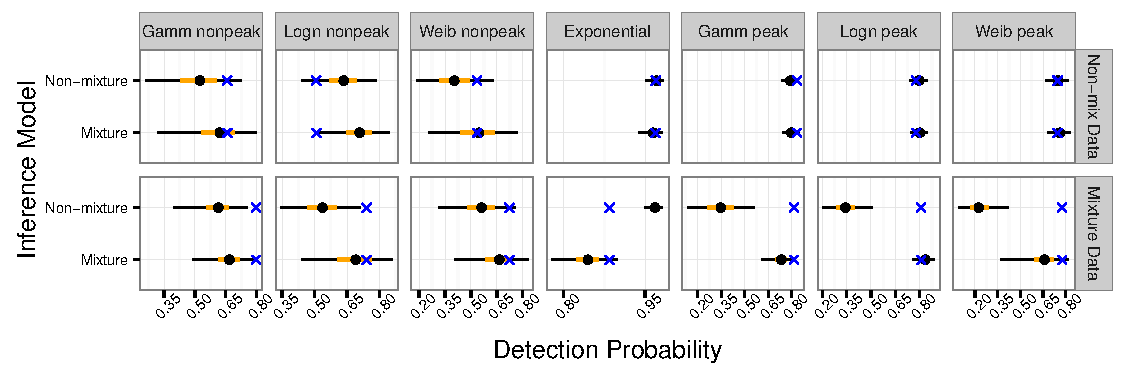
\includegraphics[width=0.98\textwidth]{Sims/SimFull/pdet_cater_correct.pdf}
\caption{\label{pdet_cater_correct} Sim3 caterpillar plots of posterior 50\% and 95\% credible intervals for the marginal probability of detection $\pdet$.  
Inference models come from the same family as the dataset but may differ in the presence/absence of a mixture component.  
Each column presents one family of simulated dataset.  
Upper plots show non-mixture datasets; lower plots show mixture datasets.  
`X' marks the expected marginal probability of detection based on true parameter values.}
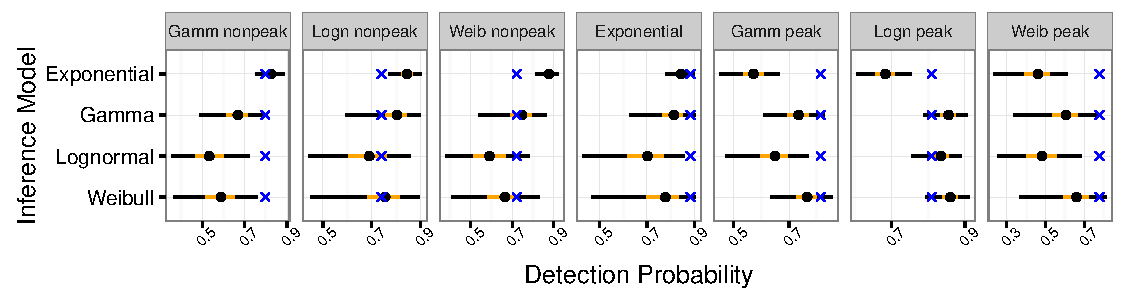
\includegraphics[width=0.98\textwidth]{Sims/SimFull/pdet_cater_family.pdf}
\caption{\label{pdet_cater_family}  Sim3 caterpillar plots of posterior 50\% and 95\% credible intervals for the marginal probability of detection $\pdet$. All data and inference models include mixtures.  
Each plot presents one simulated dataset.  
`X' marks the expected marginal probability of detection based on true parameter values.}
\end{figure}

For every dataset we simulated, estimates and credible intervals for abundance covariate coefficients $\beta^A$ were virtually the same regardless of the inference TTDD employed.  
Estimates of detection parameters $\beta^D$ varied by context.  
Comparisons of mixture and non-mixture models (like in Sim1) produced similar $\beta^D$ estimates except when fit to mixture peaked datasets, where models without a mixture component produced credible intervals twice as wide as those from mixture models with no benefit in terms of coverage.
Comparing constant-detection to time-varying models (like in Sim2), time-varying mixture TTDD models produced similar posteriors of $\beta^D$ to one another, but posteriors from the exponential mixture model were both location shifted and either narrower (exponential and nonpeaked data) or wider (peaked data).
Differences in estimates of $\beta^D$ parameters to some degree reflected differing estimation of the $\gamma$ mixing parameter -- the exponential model underestimated $\gamma$ with nonpeaked datasets and overestimated it in peaked datasets.
Many of the above patterns for nonpeaked datasets can be noted in posterior estimates from the Ovenbird data (Figure \ref{ovenposteriors}).

Results from DIC and posterior predictive checks suggested mixture models over non-mixture models for peaked data (DIC differences $>10$) and time-varying mixture TTDDs over the exponential mixture for gamma and lognormal peaked data ($>8$).
DIC preferred exponential mixtures to time-varying mixtures for exponential mixture data ($>6$); however, it also preferred the exponential mixture to time-varying mixtures (by 4-8) for lognormal nonpeaked data.  
In this last case, the posterior 95\% credible interval for $\pdet$ from the exponential mixture model did not contain the true value of $\pdet$, while the true value was within a central 60\% credible interval for all three other mixture models.  
In conjunction with Sim2 results, this last finding calls into question the utility of DIC for nonpeaked datasets.
DIC performance in Sim3 may differ from Sims 1 \& 2 not only because of the addition of fixed and random effects but also because DIC was calculated according to a different method.

%\adam{I'm guessing I should not include the following: (1) my posterior predictive pvalues are not independent; (2) for instance, for the first interval, they stay very close to 0.5-0.6 --- the models are effective at getting the first interval right; (3) likewise, a post. p-value $>$ 0.8 during the 2nd interval likely shows model misfit; all of which raises the possibility that (4) multiple simulation under the null could provide a reference distribution of posterior p-values.}

% Posterior predictive p-values for Sim1
%\begin{figure}[h!]\centering
%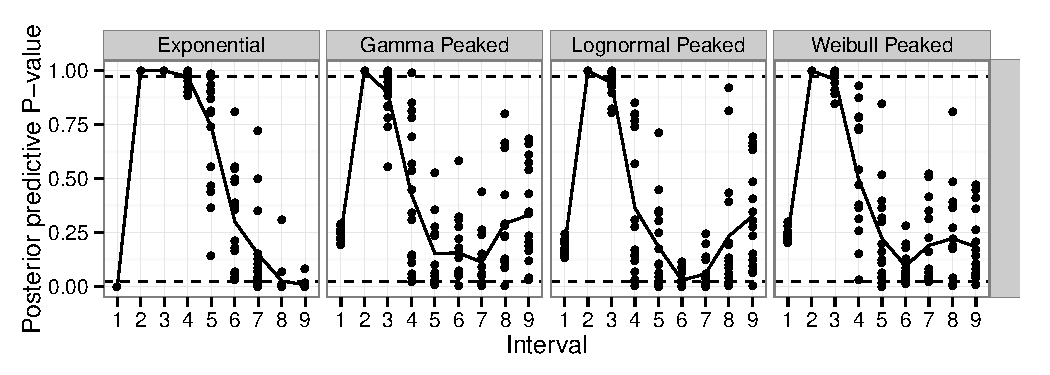
\includegraphics[width=0.78\textwidth]{Sims/SimZero/PostPredP_corr.pdf}
%\caption{\label{postpredmix} Posterior predictive p-values by interval -- Pr$\left(p_{si}^{(rep)} > p_{si}\right)$ -- for peaked mixture datasets fit with non-mixture inference models of the correct TTDD family over 16 replicates (Sim1).  
%Trendlines show mean posterior predictive p-values.  
%Dashed lines show central 95\% intervals.  
%P-values near 0 or 1 potentially indicate poor model fit.}
%\end{figure}






\section{Ovenbird analysis}\label{sec:ovenbirds}

for the Ovenbird analysis and simulations with covariates, chains were 250,000-375,000 iterations. 

\subsection{Ovenbird analysis}\label{sec:ovenbirdanalysis}

For the abundance half of our model, we used four covariates plus two random effects.  
The covariates were: (a) site age, (b) survey year, (c) an indicator of whether the site stock density is over 70\%, and (d) an indicator of whether the site experienced select-/partial-cut logging during the 1990s.  
We associated random effects with each survey year and each stand, with most stands consisting of three survey sites.  
For the detection half of our model, we used covariates for: (a) Julian date, (b) time of day, (c) temperature, (d) an indicator of whether it is the observer's first year in the database, and (e) an interaction between (a) and (d) to approximate a new observer's learning curve \citep{Alldredge2007}.  
69\% of surveys in our dataset involved observers in their first year at MNFB.  
Preliminary model fits did not support the inclusion of quadratic terms for any detection covariates.  
We associated random effects with each observer.  
We centered and standardized all continuous covariates prior to fitting models.


We fit mixture and non-mixture models from each family of TTDD to the Ovenbird dataset.  
Posterior predictive p-values by interval (Table \ref{tbl:ovencounts}) showed clear lack of fit for the non-mixture exponential model over the first three intervals.  

\begin{table}[ht]
\centering
\begin{tabular}{lccccccccc}
  \hline
Minutes & 0-2 & 2-3 & 3-4 & 4-5 & 5-6 & 6-7 & 7-8 & 8-9 & 9-10 \\ 
Count & 596 & 69 & 62 & 68 & 43 & 33 & 35 & 27 & 14 \\ 
\hline
\multicolumn{10}{l}{Posterior predictive check $p$-values by model:}\\
\hline
Expo & 0.000 & 1.000 & 1.000 & 0.347 & 0.590 & 0.372 & 0.007 & 0.006 & 0.190 \\ 
  Gamma & 0.582 & 0.820 & 0.394 & 0.006 & 0.362 & 0.637 & 0.241 & 0.519 & 0.977 \\ 
  LogNormal & 0.571 & 0.943 & 0.471 & 0.005 & 0.322 & 0.554 & 0.165 & 0.407 & 0.974 \\ 
  Weibull & 0.582 & 0.862 & 0.401 & 0.005 & 0.359 & 0.616 & 0.221 & 0.509 & 0.982 \\ 
\hline
  Exponential Mix & 0.533 & 0.804 & 0.577 & 0.021 & 0.501 & 0.668 & 0.190 & 0.338 & 0.918 \\ 
  Gamma Mix & 0.593 & 0.720 & 0.431 & 0.015 & 0.439 & 0.670 & 0.246 & 0.476 & 0.947 \\ 
  LogNormal Mix & 0.576 & 0.806 & 0.508 & 0.016 & 0.421 & 0.627 & 0.197 & 0.413 & 0.951 \\ 
  Weibull Mix & 0.596 & 0.734 & 0.411 & 0.013 & 0.421 & 0.663 & 0.252 & 0.492 & 0.958 \\ 
   \hline
\end{tabular}
\caption{\label{tbl:ovencounts} Ovenbird counts and posterior predictive p-values -- Pr$\left(D(n_i)^{(rep)} > D(n_i)^{(obs)}\right)$ -- by observation interval for each model across all surveys.  P-values near zero or one may indicate poor model fit.}
\end{table}

Figure \ref{ovenposteriors} presents caterpillar plots of posterior estimates for model parameters, overall detection probability $\pdet$, and the log10 number of Ovenbirds uncounted.  
Based on shape parameter estimates and patterns in the estimation of $\gamma$, $\beta^D$, $\pdet$, and total abundance across models, Ovenbird data most likely arose from a exponential or nonpeaked mixture TTDD.
As in Sim3, abundance covariate coefficient estimates were virtually the same across all TTDD models.  

Credible intervals for two of the abundance parameters do not contain zero, thereby suggesting notable effects.  
Select- and partial-cut logging events of the 1990s depressed local Ovenbird abundance during the study perior to roughly 25-50\% of the abundance for unlogged sites.  
Credible intervals for Site Age indicate that each decade of age increases abundance from 1.5-13\%.

DIC calculations preferred the exponential mixture TTDD to the lognormal, Weibull, and gamma mixtures (differences of 6.95, 10.7, and 11.5, respectively). These differences closely mirror those from the exponential mixture dataset in Sim3, but they also mirror those from the nonpeaked lognormal mixture dataset, where the exponential mixture 95\% credible interval for abundance did not contain the true value, and its posterior median was negatively biased by 18\% of the actual abundance.

The Ovenbird analysis highlights the ambiguity that emerged from the simulation studies: the results were entirely consistent with data generated from a finite-mixture involving a constant-rate $F_{T1}$ TTDD, but they were also consistent with finite-mixtures involving a time-varying TTDD.
Simulation results demonstrate that the exponential mixture model fits exponential mixture data well, but it does not fit time-varying mixture data well.
At this point, we have no reliable tool for differentiating field data between the two TTDD types.



\begin{figure}[h!]\centering
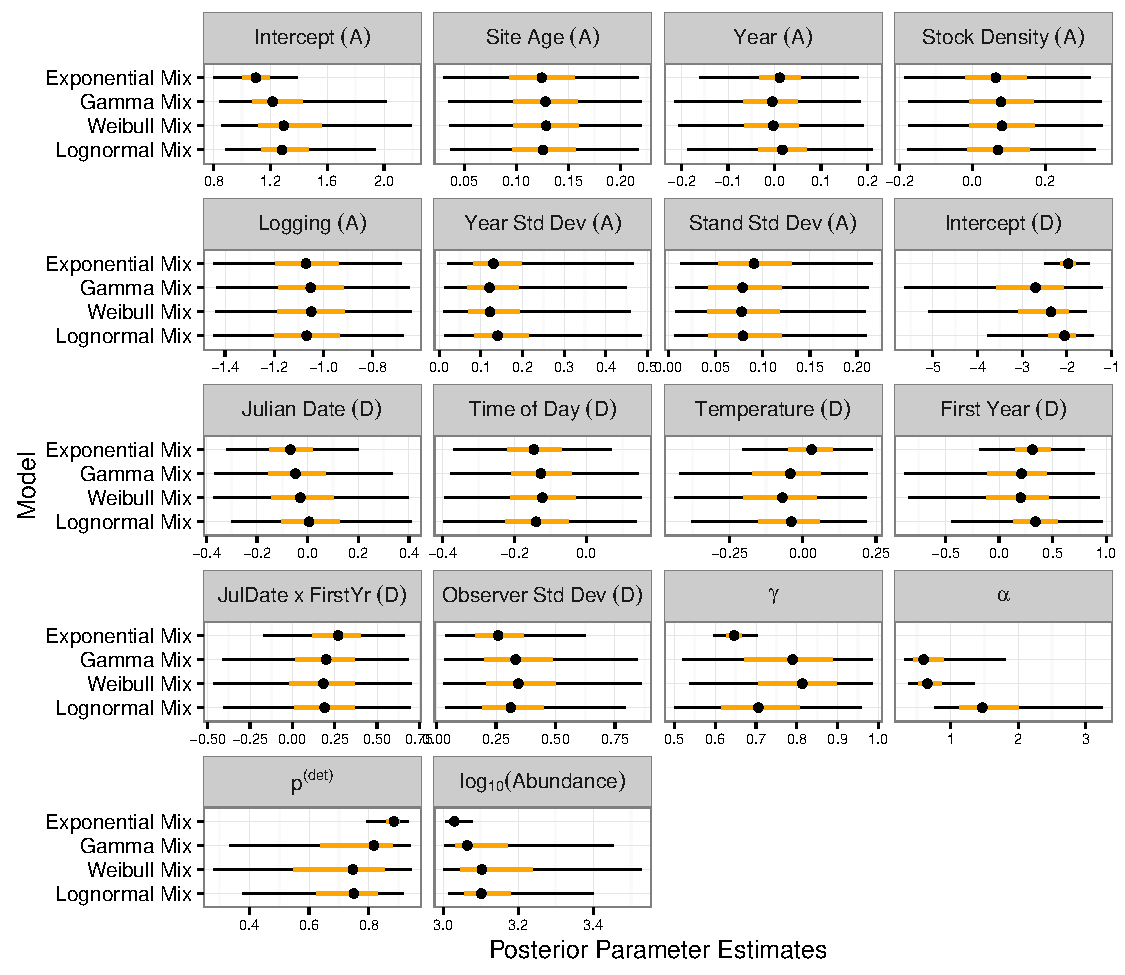
\includegraphics[width=0.88\textwidth]{OVEN/oven_sum/OVEN_Posteriors.pdf}
\caption{\label{ovenposteriors} Caterpillar plots of posterior parameter estimates for models fit to the Ovenbird data.  
Abundance and detection parameters are identified by (A) and (D), respectively.  
Gamma is the mixing parameter.  
Alpha, k, and sigma\_det are shape parameters for gamma, Weibull, and lognormal distributions, respectively.  
p\_det and log10(Uncounted) are the detection probabilty and the number of birds present but not counted across all surveys.  
Black bars are 95\% credible intervals, orange bars are 50\% credible intervals, and black dots are posterior medians.}
\end{figure}






\section{Discussion} \label{sec:discuss}

Historically, analysis of removal-sampled data assumes constant detection rates throughout the sampling period.  
This assumption provides an intuitive null model and is analytically tractable.  
However, although analysis of removal models has grown more sophisticated in recent years, the constant-detection assumption nonetheless continues unquestioned.  
We have formulated a model for non-constant detection using a time-to-event approach within a hierarchical N-mixture framework.  
Our results demonstrate that, for better or worse, the assumption of constant detection is a very strong assumption.  
When it is correct, it is the most accurate and precise of TTDD models, but when detection rates are not constant, it results in significant bias.  
Models with non-constant TTDDs, on the other hand, can adapt to a wider variety of detection patterns.

We modeled two varieties of heterogeneous detection in conjunction with one other: (i) time-varying detection rates, as modeled by non-exponential TTDDs, and (ii) detection heterogeneity among subgroups of individuals, as modeled by mixture TTDDs.  
The exponential TTDD, even when modeled with a mixture component, results in biased estimates of detection when detection actually varies with time.  
Gamma, Weibull, and lognormal TTDDs, with their extra parameter, are more accurate in handling non-constant detection data, though they are less precise when estimating data with constant detection.

The utility of applying a mixture TTDD for constant-detection models has been identified several times \citep{Pledger2000, Farnsworth2002, Alldredge2007, Reidy2011}.  
The mixture allows an analysis to account for detection heterogeneity across easy- and hard-to-detect subgroups of a population.  
Even so, some recent studies have assumed the absence of a mixture \citep{Solymos2013, Amundson2014}.  
Our study indicates that mixtures are useful even when a non-constant TTDD is used for hard-to-detect individuals.  
Models that include a mixture generally perform well even when no heterogeneity is present, but models that omit a mixture are biased and overly certain when detection heterogeneity exists.  
Indeed, for peaked datasets, mixture models can outperform non-mixture models even in the absence of heterogeneity.
% "It is tempting to choose classes of models that yield narrower confidence intervals for N; however, Coull's (1997) extensive simulation studies (summarized by Coull and Agresti (1999)) clearly reveal that this behavior can produce erroneous inferences." -- Dorazio and Royle 2003

In a limited set of situations, posterior predictive checks and DIC can identify when non-mixture or exponential TTDDs inadequately describe the marginal pattern of detections over time.  
But in many situations, neither tool points a clear way to select the correct family of TTDD.  
Given the bias that can result from assuming constant detection or omitting a mixture component, conservatism dictates that non-constant TTDDs with a mixture should be preferred.  
Among the TTDDs we considered, the mixture gamma TTDD appears to provide the best combination of accuracy and precision for nonpeaked data.  
For peaked data, gamma and Weibull models seem about equally as good.  
MCMC sampling from gamma models required from 5-10 the run time as lognormal and Weibull models.

If the estimation of effect parameters is the primary interest, then our results suggest that the exact choice of TTDD may not be important.  
Abundance effect estimates are similar regardless of the chosen TTDD, while detection effect estimates are similar for all mixture non-exponential TTDDs.  
These finding may well not hold if the same covariate is modeled in both abundance and detection models \citep{Kery2008}.

Because our focus is detection, we assumed Poisson-distributed abundance for simplicity.  
Abundance distributions that have been used to account for overdispersion include negative binomial, zero-inflated Poisson, and Poisson with survey-level random effects.  
The pattern of counts in our Ovenbird data actually reflect underdispersion, so a Conway-Maxwell Poisson distribution, which can model both overdispersion and underdispersion, may be more appropriate \citep{Wu2015}\adam{apparently, Sellers et al. (in Wu) has a comprehensive overview of the CMP.}

% Overview: Wu15
% ZIP: Etterson, Solymos12
% NB: Royle04(?)


At present, Stan does not sample discrete parameters, so the ability to marginalize out the discrete-valued latent variables $N_{s}$, as we did, can greatly facilitate MCMC sampling.

% \adam{I have contemplated on and off including a discussion of broad priors and the limit behavior as $\varphi \to 0$, but I think it's not really on topic.  
% Note: now that I've seen van Dishoeck and Manntyniemi, perhaps I should worry about informativeness in priors.}

% All estimates are based on extrapolation of the observed detections\\
% -- a) explore the tail more?  I think that'd require a lot of data\\
% -- b) requires extended observation periods or full detection data (Alldredge?)\\
% same goes for sample size

% Really, I have totally ignored the discussion of the true value of p, which I have tended to simulate in a fairly high range


To improve our choice of TTDD and/or its parameters, it makes sense to obtain more data in one of a few ways.  
One approach is to collect complete detection history records, not just first time-to-detection observations \citep{Alldredge2007}.  
This may not be feasible in studies like MNFB, where many species are observed.  
Another approach is to conduct a longer survey that better assesses the tail distribution of the TTDD; however, the longer the survey is, the greater the risk that individuals enter/depart the study area or are double-counted, which violates removal sampling assumptions \citep{LeeMarsden2008, Reidy2011}.  
A third idea is to obtain more precise time-to-detection data, even exact time-to-detection data.  
In some early explorations of our model considering just an exponential mixture TTDD, we found that credible intervals for Ovenbird detection probability were 20-25\% narrower using 9-interval surveys compared to more traditional 3-interval surveys (0-3, 3-5, and 5-10 minutes).  
For all of the above, a small pilot study may be a practical starting point.  


With the increasing use of microphone arrays for automated detection \adam{refs}, it is tempting to think TTDD models may be valuable for microphone-collected data.  
This should be the case when variations in detection result solely from organismal behaviors, such as bout singing, or if we wish to model individual random effects in the detection model.  
However, some explanations for non-constant detection are explicitly related to the observation process --- either effects of the observer on animal behavior or variations in observer effort caused by survey methodology.  
The assumption of constant detection seems more plausible in studies where observers are absent, though detection heterogeneity may still exist across subgroups of the population.

Application of TTDD modeling within the N-mixture framework should be straight-forward for other time-to-detection datasets, such as full detection-history and double-observer.  
The key difference will be in the data model, in that responses will take a different form than multinomially distributed first times to detection.  
But the underlying abundance and detection models remain the same.  
\adam{Time-heterogeneous models have been done for mark-recapture (Farcomeni and Scacciatelli 2013, who reference Hwang and Chao 2002).}

The time-to-detection approach in our model is a departure from the probability-of-detection approach that has been used in distance-removal modeling \citep{Farnsworth2005, Diefenbach2007, Solymos2013, Amundson2014}\adam{Alldredge2007?}.  
In a distance-sampling context, the probability of detection for any individual is framed as the joint probability of two independent detection events: (i) availability for detection, which occurs during an observation period with probability $P_a$, and (ii) detection of the available individual by an observer, $P_b$, also known as perceptibility \citep{Williams2002, Kery2008, Nichols2009}\adam{I haven't read Williams2002 -- cited in Royle2004.  
I'm  beginning to think this may have too-numerous antecedents to cite... in Reidy, the earliest reference is Marsh and Sinclair 1989.  
Ditto Amundson.
See also McCallum 2005.}.  
In avian point-counts, because the overwhelming majority of detections are auditory, $P_a$ is understood to be the probability that a bird vocalizes during the observation period.  
Meanwhile, perceptibility is treated as a function of distance $d$: $P_b = g(d)$, with nearby available individuals being detected with higher probability than distant individuals.  
The probability of detection is thus formulated as availability times perceptibility: $\pdet = P_aP_b$.  
Multiple studies have demonstrated that failure to incorporate distance leads to systemic bias in estimates of abundance \citep{EffordDawson2009, Solymos2013}.

The time-to-detection model as presented here in our study does not incorporate distance.  
Consequently, our definition of a TTDD necessarily represents an averaging across distance classes and a consequent loss of information if distance data are available.  
We can modify our model to account for distance.  
To be consistent with earlier distance-removal studies \citep{Farnsworth2005, Amundson2014}, we could: (i) define a time-to-\textit{availability} distribution $F_T^A(t)$ in the same manner that we have defined a TTDD in this study, (ii) modify the equation for detection probability to reflect the detection distance to individual $q$: $p_{sq}^{(det)} = g(d_q) F_T^A(C_I|\varphi_s, \boldsymbol{\theta})$, and (iii) tweak our data model accordingly.

However, our analysis makes possible a different strategy that is more consistent with a time-to-event conceptualization of the problem.  
Rather than define availability and perceptibility as independent detection events over the course of the observation period, we can define them at the event level.  
In terms of the model we have presented in this paper, this is equivalent to redefining the time-to-detection hazard function, $h_{sq}(t)$ --- which is now a function of the distance to individual $q$ --- as the product of the time-to-availability hazard function $h_{s}^A(t)$ and the perceptibility function $g(d_q)$.  
So, $h_{sq}(t) = g(d_q) h_{s}^A(t)$.  
From standard survival analysis results, $p_{sq}^{(det)} = 1 - \exp\left(-g(d_q)\int\limits_0^{C_I} h_{s}^A(u)du\right) = 1 - \left[1 - F_T^A(C_I|\varphi_s, \boldsymbol{\theta}) \right]^{g(d_q)}$.

In short, the time-to-event conceptualization frames perceptibility as a rate-of-availability multiplier rather than as a probability-of-availability multiplier.  
In a context where rates of availability are allowed to vary from individual to individual, this makes an intuitive sense --- a bird that sings twenty times during the observation period should have its overall detection probability discounted much less than a bird at the same distance which only sings once.  
This is an area of ongoing exploration.


% Skeptics of removal sampling: Johnson08, EffordDawson09, Reidy11

%\subsection{Lit Notes on Distance and Poisson Abundance}
%--- Borchers is all about this\\
%--- Farnsworth2005, EffordDawson2009, Amundson2014\\
%----- particularly noticeable with finite mixture models\\
%- Oedekoven2013 is all about covariates on distance sampling curve\\
%- necessity of using distance, too, is backed by Solymos2013, (Buckland et al 2001, 2004), Farnsworth2005, EffordDawson2009...\\
%
%Poisson assumption (do I want to discuss underdispersion?\\
%--- Denes et al 2015 discuss how Poisson assumption leads to bias in the absence of detection heterog (ref to Solymos et al 2012) or when inflated zeros are present (Joseph et al 2009) [with the obvious remedies being: NegBin and ZIP, respectively]... but is that negated by our underdispersion?\\
%
%`Unmodeled individual heterogeneity causes population size to be underestimated using capture-recapture and removal methods' (from Efford and Dawson, who cite Otis et al. 1978)\\


% Ideas for the future
% (i) Distance-removal time-to-event model
% (ii) Fit more species from this dataset over full survey duration; maybe some model selection (even Bayesian)
% (iii) Take a stab at modeling habitat
% (iv) Model for non-independent singing?
% (v) Model for density-dependent singing? (only valid, I think, if we have lots of underdispersion from(ii))
% (vi) I know I've  been warned off it, but automated detection intrigues me
% (vii) Further testing of existing model: sensitivity to priors, performance for varying detectability levels, sample size, # intervals
% (viii) Incorporate spatial random effects.  
This work has already been done, just not for TTDD models, but the real spatial dependency should be in abundance, not detection
% (ix) Comparison of methods -- just looking at my lit review, there are gadzooks strategies that people have proposed.  
Combining/comparing them seems maybe informative?  To what degree has this already been done?

\bibliography{masterbib}
\bibliographystyle{biom}



\end{document}
